\chapter{The Observer}

\vspace{1em}
\hfill
\begin{minipage}[c]{0.55\textwidth}
\raggedleft
\small\itshape
Every quantum transition taking place on every star, in every galaxy, in every remote corner of the universe, is splitting our local world into myriads of copies of itself.\\[0.5em]
\upshape\footnotesize Bryce DeWitt, ``Quantum Mechanics and Reality'' (1970)
\end{minipage}%
\hspace{0.5em}
\begin{minipage}[c]{0.12\textwidth}
% \includegraphics[width=\textwidth]{figures/ch08_observer.png}
\end{minipage}
\vspace{1.5em}

\noindent \textsc{Chapter 7 left two pictures open}. Picture A treats program-output space as a total object; Picture B keeps the observer situated with a posterior over candidate programs. In neither picture does the universal semimeasure become a distribution over observer occurrences without an additional rule.

Before turning to the observer, this chapter pauses at a nearby interpretive landmark. Everettian quantum mechanics offers a physically serious picture of multiplicity, though it is not forced by the tested formalism. The chapter then says what an observer is and identifies the self-location rule the Library does not supply.

\section*{An Everettian landmark}

There is a multiplicity much closer to hand if quantum mechanics is read in the Everettian way. The ``if'' matters.

Quantum theory is extraordinarily well confirmed. What has been argued about since the 1920s is what its formalism says exists and how definite outcomes arise. Everettian interpretations retain unitary evolution and treat decohering components of the wave function as effectively autonomous branches.\footnote{Decoherence explains the suppression of interference between relevant components and the emergence of stable quasi-classical structure. By itself it does not select one outcome, prove that branches are fundamental objects, or choose among interpretations. Everettian interpretations add an ontological reading of the unitary formalism; collapse and hidden-variable approaches read it differently.} On that reading, an observer becomes correlated with different outcomes. Calling each branch equally real is the interpretation, not an interpretation-free experimental result.

\begin{figure}[h]
\centering
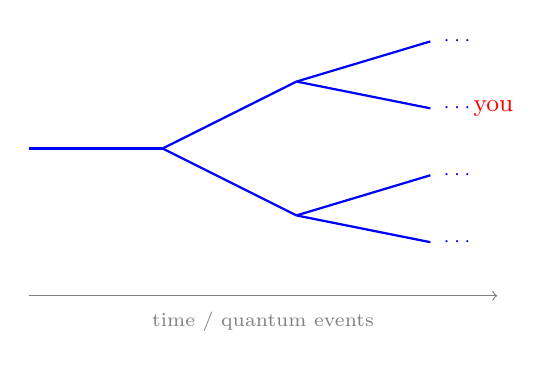
\begin{tikzpicture}[scale=0.85]
  % Trunk
  \draw[thick, blue] (0, 1) -- (2, 1);

  % First branch at t1
  \draw[thick, blue] (2, 1) -- (4, 2);
  \draw[thick, blue] (2, 1) -- (4, 0);

  % Second branches at t2
  \draw[thick, blue] (4, 2) -- (6, 2.6);
  \draw[thick, blue] (4, 2) -- (6, 1.6);
  \draw[thick, blue] (4, 0) -- (6, 0.6);
  \draw[thick, blue] (4, 0) -- (6, -0.4);

  % Continuation
  \node[font=\scriptsize, blue] at (6.4, 2.6) {$\cdots$};
  \node[font=\scriptsize, blue] at (6.4, 1.6) {$\cdots$};
  \node[font=\scriptsize, blue] at (6.4, 0.6) {$\cdots$};
  \node[font=\scriptsize, blue] at (6.4, -0.4) {$\cdots$};

  % Time axis
  \draw[->, gray] (0, -1.2) -- (7, -1.2);
  \node[font=\scriptsize, gray, anchor=north] at (3.5, -1.3) {time / quantum events};

  % "You" annotation on one branch
  \node[font=\small, red, anchor=west] at (6.5, 1.6) {you};
\end{tikzpicture}
\caption{An Everettian branching schematic. Unitary evolution correlates an observer with different outcomes, and decoherence suppresses interference between the resulting quasi-classical components. Treating those components as real branches is the Everettian interpretation; the diagram is not an interpretation-independent picture of what exists.}
\label{fig:mwi-branching}
\end{figure}

This is a landmark, not corroboration. The experiments confirm quantum predictions, not the claim that every decoherent component is a world. Everett shows that a multiplicity can be developed from a serious reading of familiar physics; it does not confirm Picture A for the Library.

If a quantum model is computably describable, its branch structure can be represented in program space. That is a relation between descriptions, not evidence that each output of each program exists. The Library and Everett therefore remain distinct proposals.

There is a deeper reason quantum mechanics belongs in this book, and it is not branching. It is weighting. The Born rule assigns outcome probabilities from squared amplitudes $|\psi|^2$. How that rule is justified and interpreted within Everett is a substantive problem; flat branch-counting is not a well-defined substitute because decoherence does not produce a unique count of branches.

This book does not derive the Born rule from the universal prior. It makes a narrower comparison (Figure~\ref{fig:born-prior}). Quantum theory assigns $|\psi|^2$ to outcomes in its own formal setting; algorithmic information theory assigns $2^{-|p|}$ to program descriptions and sums them into $M$. The domains, formulas, and warrants remain distinct.

The comparison can reveal a shared role: both attach weights to alternatives after a representation has been chosen. It does not dissolve the empirical and mathematical question of why quantum statistics follow the Born rule, and the postulate does not answer that question for us. This limited analogy is the bridge to the companion volume.

\begin{figure}[h]
\centering
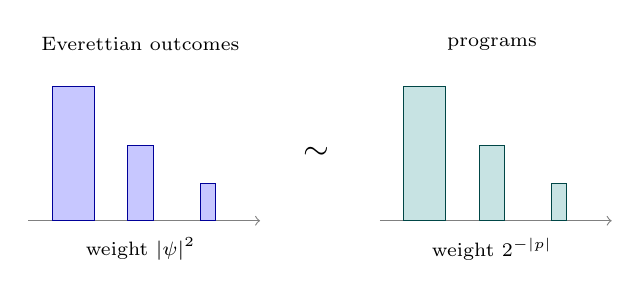
\begin{tikzpicture}[scale=0.95]
  % Left panel: Born weights on quantum branches
  \node[font=\scriptsize, anchor=south] at (1.5,2.15) {Everettian outcomes};
  \draw[->, gray] (0,0) -- (3.1,0);
  \foreach \x/\h/\w in {0.6/1.8/0.28, 1.5/1.0/0.17, 2.4/0.5/0.10} {
    \draw[draw=blue!60!black, fill=blue!22] (\x-\w,0) rectangle (\x+\w,\h);
  }
  \node[font=\scriptsize, anchor=north] at (1.5,-0.1) {weight $|\psi|^2$};

  % similarity sign
  \node[font=\large] at (3.85,0.9) {$\sim$};

  % Right panel: universal prior on programs
  \node[font=\scriptsize, anchor=south] at (6.2,2.15) {programs};
  \draw[->, gray] (4.7,0) -- (7.8,0);
  \foreach \x/\h/\w in {5.3/1.8/0.28, 6.2/1.0/0.17, 7.1/0.5/0.10} {
    \draw[draw=teal!55!black, fill=teal!22] (\x-\w,0) rectangle (\x+\w,\h);
  }
  \node[font=\scriptsize, anchor=north] at (6.2,-0.1) {weight $2^{-|p|}$};
\end{tikzpicture}
\caption{An analogy between weighting roles. Quantum theory uses Born weights $|\psi|^2$ for outcomes; algorithmic information theory weights program descriptions by $2^{-|p|}$ and sums them into $M$. The domains, formulas, and justifications differ. No Born-rule derivation or ontological identification is intended.}
\label{fig:born-prior}
\end{figure}
\FloatBarrier

\section*{What an observer is}

The chapter has used the word \emph{observer} without saying what one is. The framework needs a working definition before the next question makes sense.

For the purposes of this framework, an observer is modeled as a local pattern within some candidate $U(p)$, with internal organization, a sensorium, memory, and a capacity to model. An Everettian may place such a pattern within a decoherent branch. This is a working model, not a solution to the hard problem of consciousness or a claim that every observer is literally computable.

But not every substructure is an observer, and among those that are, a distinction matters. An observer-moment, a configuration that merely \emph{matches} an observer-state for an instant, can occur almost anywhere. An observer whose inference \emph{works}, who can model its surroundings, persist, and do science, needs something specific from the universe it is in.

\emph{Hierarchical decomposability.} An observer's predictions, models, and actions all rely on isolating subsystems. The cell can be modeled without the quarks. The apple's fall can be predicted without the wave function of every electron. For this to work at all, the universe (whether $U(p)$ or the relevant branch of the wave function) must have a hierarchical structure: at each scale, local short programs approximate local substructures well enough for the observer to reason. Without this, no observer could build a model that reliably tracks anything.

This is a strong restriction on which candidate programs support observers of that kind. Many computable outputs are locally chaotic, tightly coupled, or homogeneous and do not admit effective local modeling. There is no canonical way to count all programs, so the book makes no claim about what a ``vast majority'' of them are like.

A caveat the rest of the chapter will sharpen: none of this says observer-\emph{states} cannot occur in the lawless majority. They can. In a large enough chaotic or high-entropy structure, a configuration matching your exact observer-state can fluctuate into being for a moment, carrying all your apparent memories and none of the lawful past they seem to record. That is the Boltzmann brain, one of the uncomfortable things the framework permits, and we return to it below. The decomposability requirement is not a condition for an observer-state to \emph{exist}; it is what an observer needs for its inference to \emph{work}, for its models to track its world, for it to persist past the instant.

Our observed environment is locally decomposable at multiple scales. The success of effective theories is evidence for that feature of our environment. It is not evidence that an observer measure is concentrated there, because the framework has supplied no observer measure.

\emph{Local inference.} The observer's epistemic activity, science, is not a search for the global program. Kolmogorov complexity is uncomputable, and an observer with finite resources could not carry out global Solomonoff induction even approximately without choosing severe bounds. What the observer does instead is build a collection of tractable local models $p_s$, each approximating a local substructure $s$. These are the effective theories of physics, the models of biology, the heuristics of everyday cognition. Together they form the observer's working model of its local region.

The observer never has access to the global program. The observer has access to a prefix of its local substructure, restricted to whatever its sensorium can resolve. From this, it infers local $p_s$'s and predicts forward. The relevant ensemble is not a posterior over global programs; it is the collection of local effective theories the observer maintains.

This is what science is, in this framework. Not the discovery of \emph{the} program. The construction of a library of local approximations, scale by scale, each anchored to a substructure the observer can probe.

\emph{The self as a local model.} The same picture extends to the observer's self-representation. The brain's model of itself is a short local program approximating the substructure the observer occupies. $I$ is one of the local theories. The dissolution of the self in Chapter 14 follows from this: the self-model is not different in kind from the other local effective theories the observer maintains. The self is a $p_{\text{self}}$, useful, finite, approximate, and like every other $p_s$, not the structure it describes.

With these in place, the question of the next section sharpens. The observer is locally modeled, with no access to a global view. So: what can the posterior over programs tell you, and what extra structure would be needed to ask which occurrence is \emph{you}?

\section*{Where am I?}

Under Picture A or an Everettian ontology, a sharp question emerges. Suppose several observer occurrences match your current self-description: your memories, sensory state, and moment of reading this. What would make one of them your self-location? (Figure~\ref{fig:where-am-i}.)

\begin{figure}[h]
\centering
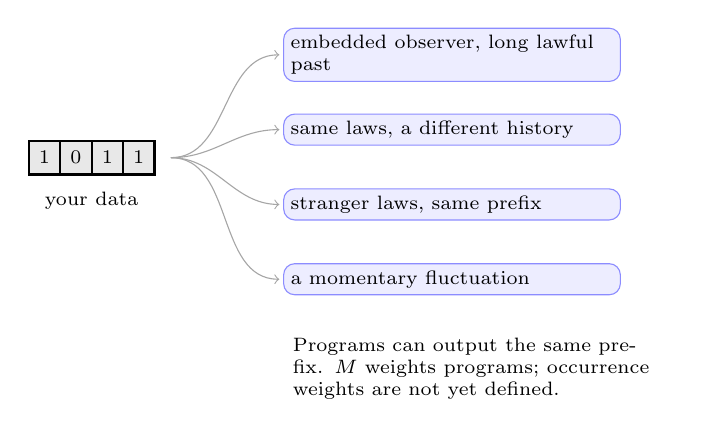
\begin{tikzpicture}[scale=0.95]
  % data prefix (left)
  \foreach \i/\b in {0/1, 1/0, 2/1, 3/1} {
    \draw[thick, fill=gray!18] (\i*0.42,0.9) rectangle (\i*0.42+0.42,1.35);
    \node[font=\scriptsize] at (\i*0.42+0.21,1.125) {\b};
  }
  \node[font=\scriptsize, anchor=north] at (0.84,0.8) {your data};
  % candidate worlds (right)
  \foreach \y/\lbl in {2.5/{embedded observer, long lawful past}, 1.5/{same laws, a different history}, 0.5/{stranger laws, same prefix}, -0.5/{a momentary fluctuation}} {
    \node[font=\scriptsize, anchor=west, draw=blue!45, rounded corners, inner sep=2.5pt, fill=blue!7, text width=4.1cm] at (3.4,\y) {\lbl};
    \draw[->, gray!70] (1.9,1.125) to[out=0,in=180] (3.35,\y);
  }
  \node[font=\scriptsize, anchor=north west, text width=5.0cm] at (3.4,-1.15) {Programs can output the same prefix. $M$ weights programs; occurrence weights are not yet defined.};
\end{tikzpicture}
\caption{Two underdeterminations. A finite stretch of data (left) is compatible with many candidate programs (right), and $M$ gives a posterior over those programs. If several observer occurrences match the same data, $M$ alone does not distribute probability among them. ``Which program predicts next?'' and ``which occurrence am I?'' are different questions.}
\label{fig:where-am-i}
\end{figure}

The literature has attempted to answer this with indexical assumptions. The \emph{Self-Sampling Assumption} (SSA) says to reason as if you are a random sample from a specified reference class. The \emph{Self-Indication Assumption} (SIA) treats your existence as evidence favoring hypotheses with more eligible observers. Other approaches use a xerographic distribution that assigns first-person weights directly. These proposals disagree about cases such as Sleeping Beauty, the doomsday argument, and Boltzmann observers. None is forced, and each must say what counts as an occurrence.

The book does not commit to an indexical assumption. So \emph{where am I?}, understood as self-location among occurrences, does not merely have a broad posterior here; it is undefined until extra structure is supplied. That is a limit of the framework, kept visible rather than hidden inside $M$.

There is a deeper underdetermination underneath this one, and it is worth naming because Chapter 6 promised it. The book has been speaking in two pictures without choosing between them. In Picture A, program-output space is treated as a static object carrying program-description weights. In Picture B, you are situated with access only to finite local data and a posterior over candidate programs. The question of which picture is \emph{real}, whether the totality is ontic or only the situated predictive use is warranted, has no answer supplied by $M$. The postulate declines to privilege either decomposition. The book therefore holds the ontology open.

The framework cannot settle self-location without a rule it does not contain. One hope remains: perhaps a greater mind could supply a uniquely correct overview. The next chapter asks what such an overview would mean, and finds no privileged view at the top.
